\fontsize{9}{10.5}\selectfont
\par\Needspace{100pt}\section*{Older Q3: Architecture, NFRs and patterns}\label{older-q3}
\phantomsection\addcontentsline{toc}{section}{Older Q3: Architecture, NFRs and patterns}
\markboth{Older papers | Q3}{}
\textbf{Shared method:} use \hyperref[answer-architecture]{A, p.\ \pageref{answer-architecture}}, \hyperref[shared-pattern]{P, p.\ \pageref{shared-pattern}}, \hyperref[answer-mvc]{M, p.\ \pageref{answer-mvc}} and \hyperref[answer-pattern-cost]{C, p.\ \pageref{answer-pattern-cost}}. The case answers supply the concrete responsibilities, constraints and trade-offs.
\par\Needspace{85pt}\subsection*{AY2022/23 S1: Car sales --- Q3 (25 marks)}\label{old-2223-s1-q3}

\sectionlabel{h-q3--architecture-and-pattern-composition-25-marks}
\textbf{(a)(i) Architecture and detailed classes (8); (ii) alternative using a different pattern and its advantages (6). (b)(i) Combined-pattern car-sales scenario and classes (8); (ii) when patterns can be combined/\allowbreak{}merged, with an example (3).}


\textbf{(a)(i)} Apply the shared layered frame. HoldController enforces allocation/\allowbreak{}refund rules rather than putting them into the page. Extend Q2's conceptual model as follows:







\par\smallskip\noindent\begin{minipage}{\linewidth}\centering
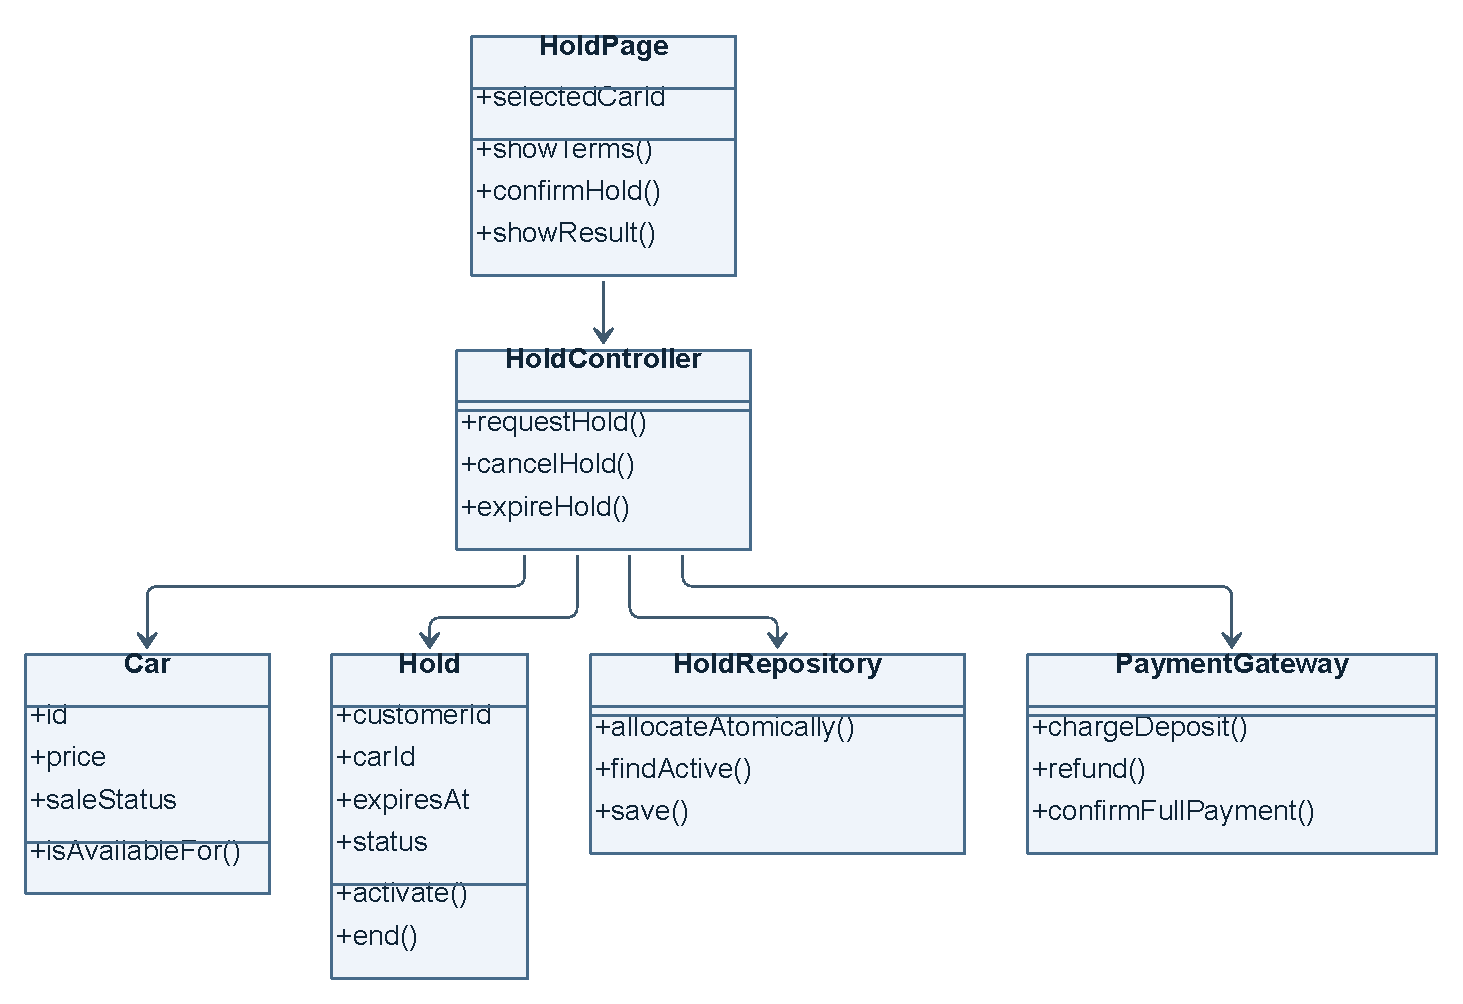
\includegraphics[width=408.22pt]{images/fig-051.pdf}
\captionof{figure}{Car sales: Q3 --- Architecture and pattern composition (25 marks)}\end{minipage}\par\smallskip

\begin{studycolumns}
\vspace{0pt}





Order/\allowbreak{}delivery controls similarly require full-payment confirmation before delivery. Persistence must enforce active-hold uniqueness; payment callbacks need reconciliation to avoid recording inconsistent states.

\textbf{(a)(ii)} Apply \hyperref[answer-mvc]{M, p.\ \pageref{answer-mvc}}. Model: Car/Hold plus services; Views: listing/details/status screens; Controller: HoldController. Notify both staff and customers when hold state changes; layered persistence can remain.

\textbf{(b)(i)} Combine \textbf{Strategy} with \textbf{Simple Factory} for selecting a dealer payment provider. This is a proposed extension; the appendix only requires integration with the dealer payment system.


\textbf{Class diagram:} use \hyperref[shared-pattern]{P, p.\ \pageref{shared-pattern}}. Context = \code{Hold\allowbreak{}Controller}; Strategy = \code{Payment\allowbreak{}Strategy}; Factory = \code{Payment\allowbreak{}Factory}. Concrete strategies: \code{Card\allowbreak{}Payment}, \code{Wallet\allowbreak{}Payment}. Interface/concrete operations: \code{charge()}, \code{refund()}. Provider selection is a proposed extension; retain availability, allocation and refund rules.



Patterns do not replace validation or transaction handling.

\textbf{(b)(ii)} Use \hyperref[answer-pattern-cost]{C, p.\ \pageref{answer-pattern-cost}}. MVC combines Observer/Strategy; the payment example separates behaviour from construction. Shared classes are acceptable when responsibilities stay clear.
\end{studycolumns}

\par\Needspace{85pt}\subsection*{AY2022/23 S2: Shopping chatbot --- Q3 (25 marks)}\label{old-2223-s2-q3}

\sectionlabel{h-q3--chatbot-architecture-and-combined-patterns-25-marks}
\textbf{(a)(i) Architecture/\allowbreak{}detailed classes (8); (ii) alternative pattern and advantages (6). (b)(i) Combined patterns and class diagram (8); (ii) structural method for comparing architectures (3).}


\textbf{(a)(i)} Apply the shared layered frame with a gateway to the existing shop. Keep order/\allowbreak{}replacement decisions in deterministic services; natural-language interpretation identifies the requested operation.




\par\smallskip\noindent\begin{minipage}{\linewidth}\centering
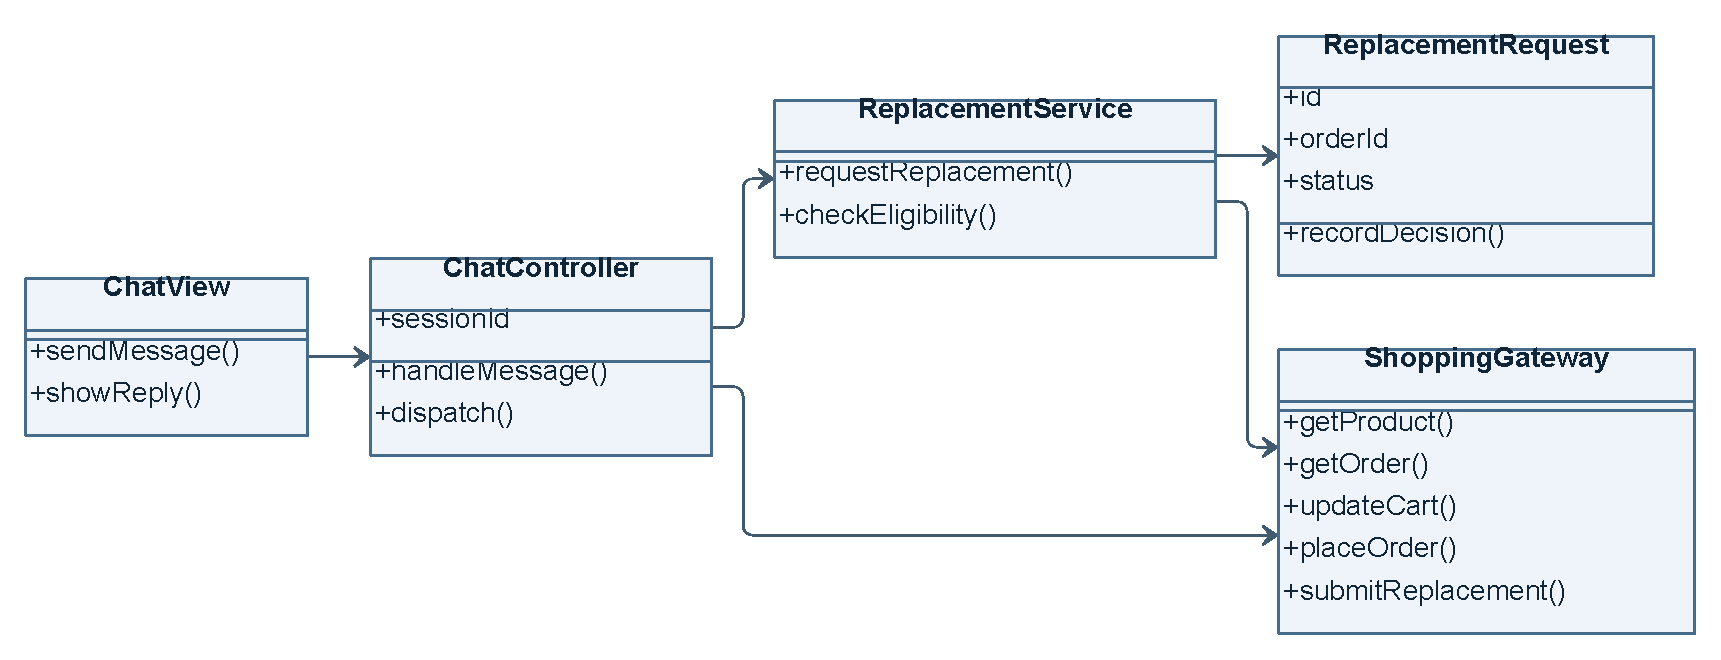
\includegraphics[width=484.44pt]{images/fig-056.pdf}
\captionof{figure}{Shopping chatbot: Q3 --- Chatbot architecture and combined patterns (25 marks)}\end{minipage}\par\smallskip

\begin{studycolumns}
\vspace{0pt}



\textbf{(a)(ii)} Apply \hyperref[answer-mvc]{M, p.\ \pageref{answer-mvc}}. Models: conversation/cart/replacement request; Views: chat and order status; Controllers: input handling. Notify both views when the company decision arrives; retain layered services underneath.

\textbf{(b)(i)} Combine Strategy for handling different intents with Simple Factory for selecting the handler:


\textbf{Class diagram:} use \hyperref[shared-pattern]{P, p.\ \pageref{shared-pattern}}. Context = \code{Chat\allowbreak{}Controller}; Strategy = \code{Intent\allowbreak{}Handler}; Factory = \code{Handler\allowbreak{}Factory}. Concrete strategies: \code{Product\allowbreak{}Query\allowbreak{}Handler}, \code{Replacement\allowbreak{}Handler}, \code{Refund\allowbreak{}Handler}. Interface/concrete operations: \code{execute()}. The chatbot selects behaviour; the existing shop still makes the company approval decision.





\textbf{(b)(ii)} Use \hyperref[answer-architecture]{A, p.\ \pageref{answer-architecture}}: compare cohesion, coupling, cycles and change propagation. A changed shopping API should affect its gateway, not every handler/view; raw class/edge counts alone prove little.
\end{studycolumns}

\par\Needspace{85pt}\subsection*{AY2023/24 S1: DevSecOps --- Q3 (25 marks)}\label{old-2324-s1-q3}


\begin{studycolumns}
\vspace{0pt}
\sectionlabel{h-q3--quality-attributes-and-architecture-25-marks}
\textbf{(a)(i) Important NFRs (6); (ii) detailed architecture/\allowbreak{}classes addressing them (8). (b)(i) Combined-pattern scenario/\allowbreak{}classes (6); (ii) can AI design software architectures? (5).}


\textbf{(a)(i)} Apply \hyperref[answer-architecture]{A, p.\ \pageref{answer-architecture}} to three proposed NFRs: source confidentiality/isolated execution; replaceable interoperable engines; responsive, reliable long-running scans. Agree measurable criteria rather than inventing guaranteed numbers.

\textbf{(a)(ii)} Add plug-in engine boundaries to the shared layered frame. A scan coordinator implements a Facade for the UI; a stable Engine interface supports replacement tool adapters. Proposed queued jobs and isolated execution address responsiveness and fault containment.
\end{studycolumns}


\par\smallskip\noindent\begin{minipage}{\linewidth}\centering
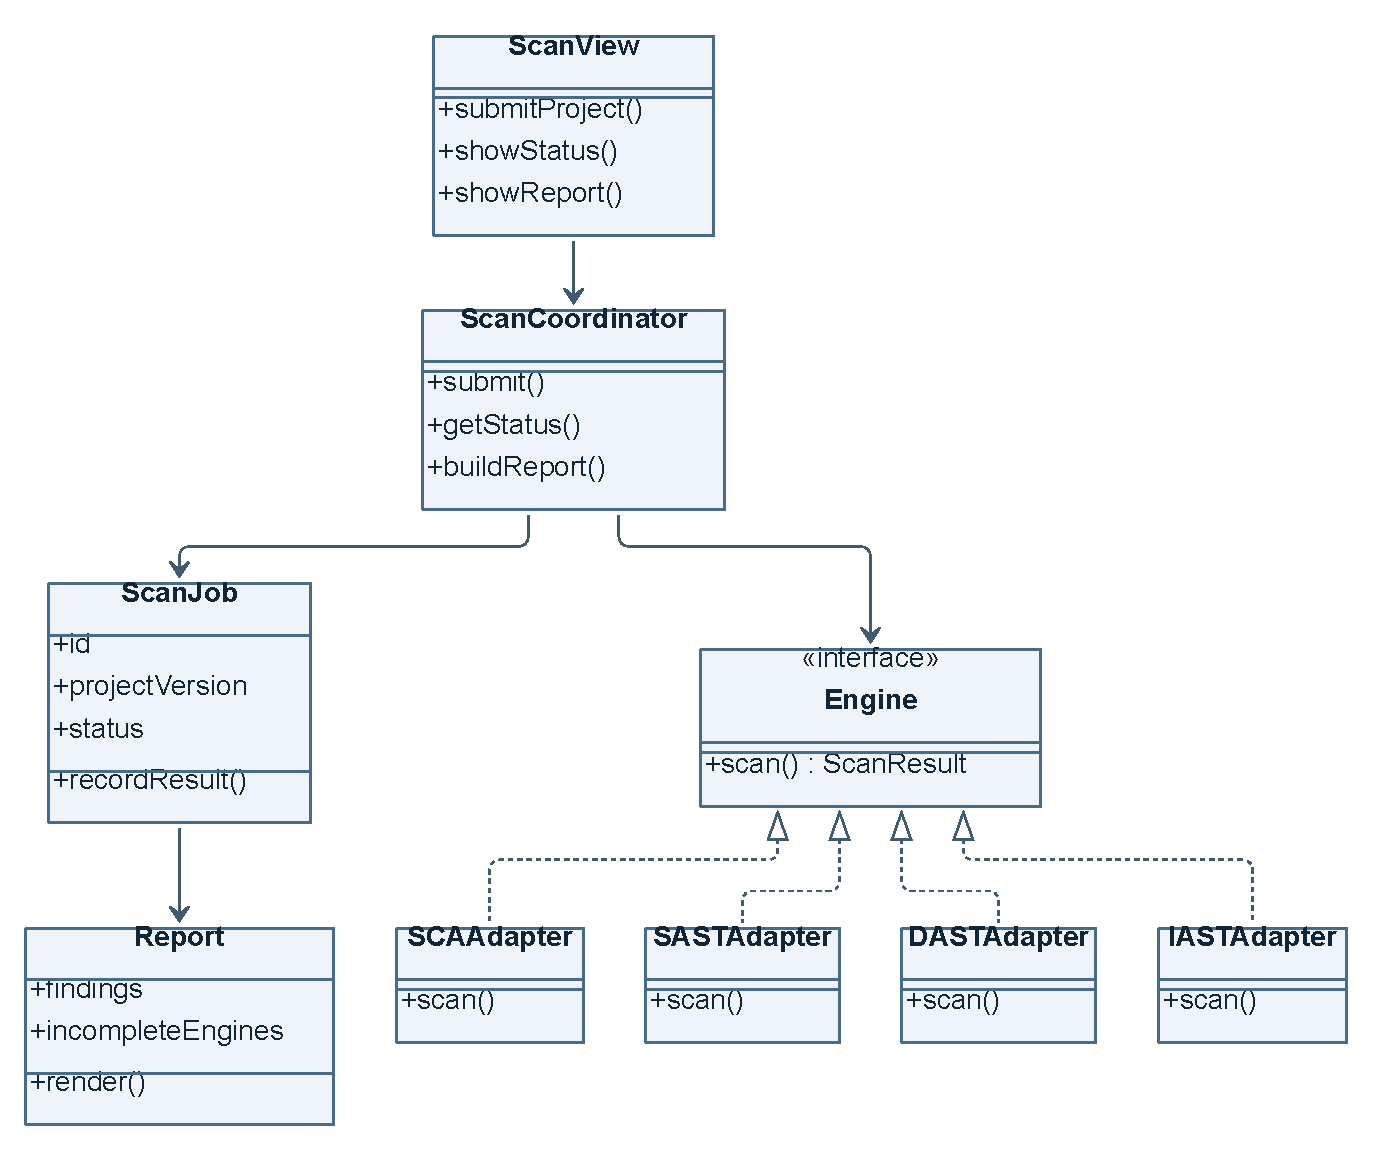
\includegraphics[width=386.32pt]{images/fig-061.pdf}
\captionof{figure}{DevSecOps: Q3 --- Quality attributes and architecture (25 marks)}\end{minipage}\par\smallskip

\begin{studycolumns}
\vspace{0pt}




Isolate source access and credentials at adapter/\allowbreak{}execution boundaries; apply timeouts and preserve partial-failure information. Adding an engine should add an adapter rather than change UI or report-domain rules. These choices directly connect the architecture to the proposed NFRs.

\textbf{(b)(i)} Combine Strategy and Simple Factory: engines share the Engine contract while an EngineFactory creates configured adapters. ScanCoordinator uses the resulting strategies without knowing their concrete classes.


\textbf{Class diagram:} use \hyperref[shared-pattern]{P, p.\ \pageref{shared-pattern}}. Context = \code{Scan\allowbreak{}Coordinator}; Strategy = \code{Engine}; Factory = \code{Engine\allowbreak{}Factory}. Concrete strategies: \code{SASTAdapter}, \code{SCAAdapter}, \code{DASTAdapter}, \code{IASTAdapter}. Interface/concrete operations: \code{scan()}. Create configured tool adapters; preserve the engine result/partial-failure contract.





\textbf{(b)(ii)} AI can propose candidate NFRs, architectures, diagrams and trade-offs. It cannot set missing stakeholder priorities or prove security/performance/integration fitness. Ground it in requirements, review traceability and validate risky decisions with prototypes/tests and human judgement.
\end{studycolumns}

\par\Needspace{85pt}\subsection*{AY2023/24 S2: CodeAgent --- Q3 (25 marks)}\label{old-2324-s2-q3}


\begin{studycolumns}
\vspace{0pt}
\sectionlabel{h-q3--extending-codeagent-and-architecture-25-marks}
\textbf{(a)(i) Two additional agent roles (3); (ii) one important NFR (3); (iii) detailed architecture addressing it (8). (b)(i) Combined-pattern scenario/\allowbreak{}classes (6); (ii) can CodeAgent replace development teams? (5).}


\textbf{(a)(i)} A \textbf{Test Engineer agent} creates/\allowbreak{}executes candidate regression tests and reports evidence; a \textbf{Requirements Analyst agent} clarifies requests and checks traceability between requirements and reviewed changes. These are proposed additions, distinct from the existing conversation-focused QA-Checker.

\textbf{(a)(ii)} Choose \textbf{extensibility/\allowbreak{}maintainability}: new agent roles and analysis strategies should be addable without changing all existing agents. The request to introduce roles makes this a defensible priority; correctness/\allowbreak{}security would also require attention in a real platform.

\textbf{(a)(iii)} Use layered UI/\allowbreak{}orchestration/\allowbreak{}domain boundaries with plug-in agents. A coordinator schedules phases and supervised conversations; agents implement a common contract; configuration/\allowbreak{}registry selects roles. This avoids hard-coded peer dependencies throughout the UI.
\end{studycolumns}


\par\smallskip\noindent\begin{minipage}{\linewidth}\centering
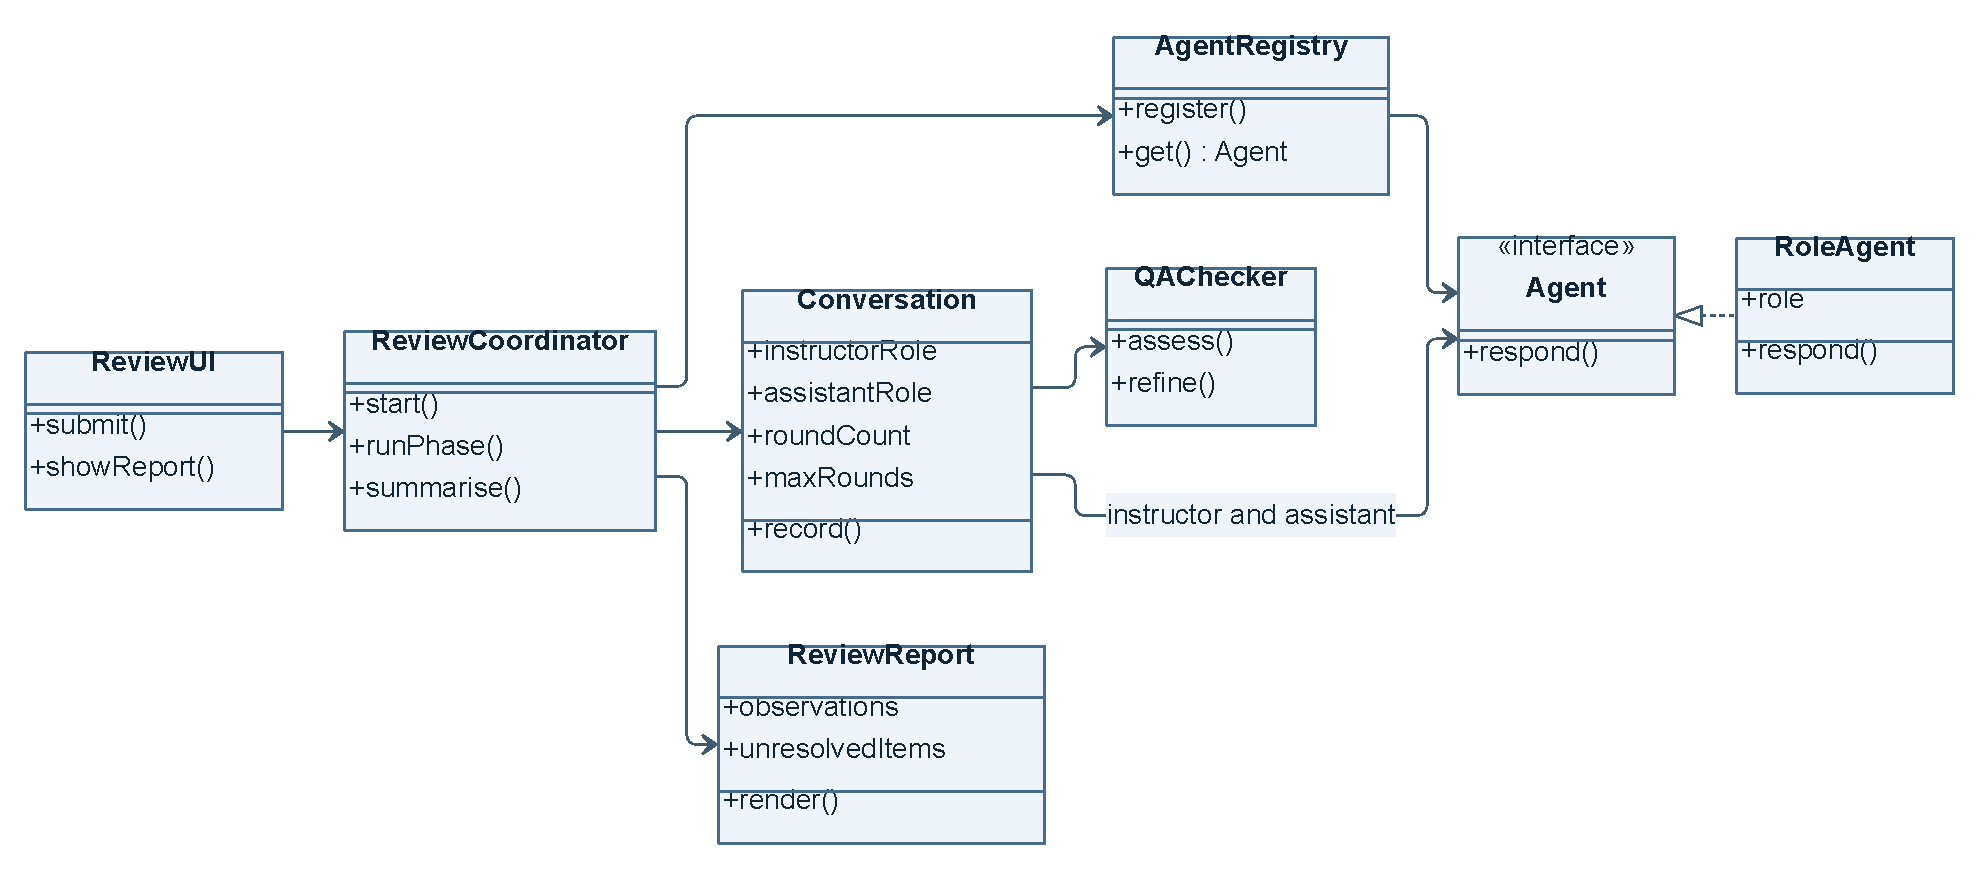
\includegraphics[width=514.00pt]{images/fig-067.pdf}
\captionof{figure}{CodeAgent: Q3 --- Extending CodeAgent and architecture (25 marks)}\end{minipage}\par\smallskip

\begin{studycolumns}
\vspace{0pt}



Configure RoleAgent for User/\allowbreak{}CEO/\allowbreak{}CPO/\allowbreak{}CTO/\allowbreak{}Reviewer/\allowbreak{}Coder, or add new Agent implementations. Persist logs and preserve unresolved status when conversation limits are reached. The registry approach supports the chosen extensibility NFR; storage and orchestration should not depend on one concrete role.

\textbf{(b)(i)} Combine Strategy for analysis methods with Simple Factory for constructing the requested checks:


\textbf{Class diagram:} use \hyperref[shared-pattern]{P, p.\ \pageref{shared-pattern}}. Context = \code{Reviewer\allowbreak{}Agent}; Strategy = \code{Review\allowbreak{}Check}; Factory = \code{Check\allowbreak{}Factory}. Concrete strategies: \code{Consistency\allowbreak{}Check}, \code{Vulnerability\allowbreak{}Check}, \code{Format\allowbreak{}Check}. Interface/concrete operations: \code{analyse()}. Choose the requested review check without hard-coding it in the reviewer.



Reviewer's three analyses retain separate responsibilities, while creation is centralised. A new check can be registered without duplicating the review workflow.

\textbf{(b)(ii)} CodeAgent assists review/revision, but does not replace stakeholder negotiation, requirements clarification, architecture judgement, independent validation, operations or accountability. Agent agreement is not proof of correct software; accept changes using reviewed outputs and executable tests.
\end{studycolumns}

